% Number of roots of X^3-2 mod p for the 17982 primes 3<p<200000, against Chebotarev's 1/6, 1/2, 1/3 (generated).
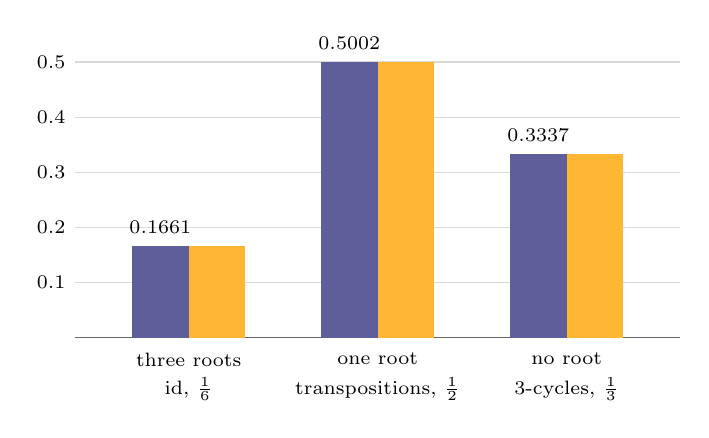
\begin{tikzpicture}[yscale=7,xscale=2.4]
\draw[black!60] (0.4,0)--(3.6,0);
\draw[black!15] (0.4,0.1)--(3.6,0.1); \node[font=\scriptsize,anchor=east] at (0.4,0.1) {$0.1$};
\draw[black!15] (0.4,0.2)--(3.6,0.2); \node[font=\scriptsize,anchor=east] at (0.4,0.2) {$0.2$};
\draw[black!15] (0.4,0.3)--(3.6,0.3); \node[font=\scriptsize,anchor=east] at (0.4,0.3) {$0.3$};
\draw[black!15] (0.4,0.4)--(3.6,0.4); \node[font=\scriptsize,anchor=east] at (0.4,0.4) {$0.4$};
\draw[black!15] (0.4,0.5)--(3.6,0.5); \node[font=\scriptsize,anchor=east] at (0.4,0.5) {$0.5$};
\fill[MidnightBlue!70] (0.70,0) rectangle (1.00,0.1661);
\fill[Orange!80] (1.00,0) rectangle (1.30,0.1667);
\node[font=\scriptsize,anchor=north] at (1,-0.01) {three roots};
\node[font=\scriptsize,anchor=north] at (1,-0.055) {$\mathrm{id}$, $\frac16$};
\node[font=\scriptsize,anchor=south] at (0.85,0.1711) {$0.1661$};
\fill[MidnightBlue!70] (1.70,0) rectangle (2.00,0.5002);
\fill[Orange!80] (2.00,0) rectangle (2.30,0.5000);
\node[font=\scriptsize,anchor=north] at (2,-0.01) {one root};
\node[font=\scriptsize,anchor=north] at (2,-0.055) {transpositions, $\frac12$};
\node[font=\scriptsize,anchor=south] at (1.85,0.5052) {$0.5002$};
\fill[MidnightBlue!70] (2.70,0) rectangle (3.00,0.3337);
\fill[Orange!80] (3.00,0) rectangle (3.30,0.3333);
\node[font=\scriptsize,anchor=north] at (3,-0.01) {no root};
\node[font=\scriptsize,anchor=north] at (3,-0.055) {$3$-cycles, $\frac13$};
\node[font=\scriptsize,anchor=south] at (2.85,0.3387) {$0.3337$};
\end{tikzpicture}
